\documentclass[11pt]{article}
\usepackage[utf8]{inputenc}
\usepackage{amsmath}
\usepackage{amssymb}
\usepackage{algpseudocode}
\usepackage{listings}
\usepackage{xcolor}
\usepackage{booktabs}
\usepackage{graphicx}
\usepackage{hyperref}
\usepackage{geometry}
\usepackage{titlesec}
\usepackage{enumitem}
\usepackage{booktabs}
\usepackage{forest}
\usepackage{tikz}
\usepackage{import} 
\usepackage[ruled,vlined]{algorithm2e}
\usetikzlibrary{calc, positioning, arrows.meta}
\geometry{a4paper, margin=1in}
\titleformat{\section}{\large\bfseries}{\thesection}{1em}{}
\titleformat{\subsection}{\normalsize\bfseries}{\thesubsection}{1em}{}

\definecolor{codegreen}{rgb}{0,0.6,0}
\definecolor{codegray}{rgb}{0.5,0.5,0.5}
\definecolor{codepurple}{rgb}{0.58,0,0.82}
\definecolor{backcolour}{rgb}{0.95,0.95,0.92}

\lstset{
    language=C++,
    backgroundcolor=\color{backcolour},   
    commentstyle=\color{codegreen},
    keywordstyle=\color{magenta},
    numberstyle=\tiny\color{codegray},
    stringstyle=\color{codepurple},
    basicstyle=\ttfamily\footnotesize,
    breakatwhitespace=false,         
    breaklines=true,                 
    captionpos=b,                    
    keepspaces=true,                 
    numbers=left,                    
    numbersep=5pt,                  
    showspaces=false,                
    showstringspaces=false,
    showtabs=false,                  
    tabsize=4,
    frame=lines,
}

\begin{document}

\begin{center}
    \centering
    {\Huge \textbf{CSC3060 Project 1 Report}} \\[0.5cm]
    
    \textbf{Student Name} \quad Chaoyi, Sun \\[0.1cm]
    \textbf{Student ID} \quad 124090550 \\[1cm]
\end{center}

\section{Theoretical Foundation}

\subsection{Binary Addition Principle}
Binary addition can be decomposed into two components:
\[
    A + B = \text{sum without carry (Sum)} + \text{carry propagation (Carry)}
\]

\begin{center}
\begin{tabular}{cccc}
\toprule
\textbf{A} & \textbf{B} & \textbf{Sum} & \textbf{Carry} \\
\midrule
0 & 0 & 0 & 0 \\
0 & 1 & 1 & 0 \\
1 & 0 & 1 & 0 \\
1 & 1 & 0 & 1 \\
\bottomrule
\end{tabular}
\par\vspace{5pt}
\textbf{Truth Table for Binary Addition}
\end{center}
If a bit position does not generate a carry (i.e., at most one of the two bits is 1), the result can be represented by $A \oplus B$. Otherwise, if both bits are 1, a carry is generated, which is captured by $A \& B$.
\vspace{3pt}\\
The generated carry must be propagated to the next higher bit position, which is achieved by left-shifting the carry by 1. Since a carry generated in one bit position can propagate to higher bits, the algorithm iteratively processes the sum and carry until no further carries remain.
\vspace{8pt}\\
\begin{algorithm}[H]
\caption{Addition via Bitwise Operations}
\KwIn{Two integers $a$ and $b$}
\KwOut{The sum $a + b$}

\While{$b \neq 0$}{
    $\text{sum} \gets a \oplus b$ \\
    $\text{carry} \gets (a \& b) \ll 1$ \\
    $a \gets \text{sum}$  \\
    $b \gets \text{carry}$ 
}
\Return{$a$}
\end{algorithm}

\subsection{Negate}
All implementations based on signed integers using two's complement representation:
\[
-x = \sim x + 1
\]
where $\sim x$ denotes bitwise NOT operation.
\newpage
\textbf{Proof} 

The formula can be derived from two fundamental identities:

\[
\begin{cases}
x + (-x) = 0 \quad &\text{(definition of additive inverse)} \\[4pt]
x + (\sim x) = -1 \quad &\text{(bitwise complement yields all ones)}
\end{cases}
\]

Subtracting the second equation from the first gives:
\[
[x + (-x)] - [x + (\sim x)] = 0 - (-1) \;\Longrightarrow\; -x - (\sim x) = 1 \;\Longrightarrow\; -x = \sim x + 1.
\]

Thus, the negative of any integer can be obtained by flipping all bits and adding one.

\subsection{Comparison}
Since the comparison operators is not allowed in the project, their relative magnitude can be determined by analyzing the sign bit of their difference. Specifically:
\[
\text{sgn}(a - b) = 
\begin{cases}
0 & \text{if } a \geq b \\
1 & \text{if } a < b
\end{cases}
\]
where $\text{sgn}(x)$ is implemented as the bitwise operation $(x \gg 31) \& 1$.

\subsection{Type Casting}
The algorithm casts operands to \texttt{uint32\_t} to prevent signed integer overflow (e.g., \texttt{abs(INT\_MIN)}), while reusing helper functions like \texttt{add} that expect \texttt{int32\_t} arguments. 
\vspace{3pt}\\
This approach is valid because \texttt{static\_cast} between same-width integers purely \textbf{reinterprets} the bit pattern without generating runtime instructions or altering the bits. 
\vspace{3pt}\\
Furthermore, since the helper functions rely exclusively on bitwise operations, which are agnostic to the sign bit, the binary logic remains correct regardless of type interpretation.
\newpage
\section{Function Implementations}
\subsection{Addition}

Let $W=32$ denote the bit width. Subsequent analyses are implicitly based on $W$-bit signed integers.
\vspace{3pt}\\
As established in Section~1.1, the operation requires at most $W$ iterations.
\vspace{3pt}
\begin{lstlisting}[language=C++]
carry = (a & b) << 1;
a = a ^ b;
b = carry;
\end{lstlisting}
\vspace{8pt}
Thus, the addition operation can be achieved in $O(W)$ time complexity using the aforementioned operations.
\vspace{5pt}\\
However, in this algorithm, each step depends on the value generated in the previous iteration, raising the question of whether carry propagation can be computed in parallel. Modeling the computation as a tree structure allows us to apply a recursive doubling approach, effectively optimizing the carry propagation. (Similar to $\textbf{Carry Lookahead Adder}$ mentioned in the lecture.)
\vspace{10pt}\\
\resizebox{\textwidth}{!}{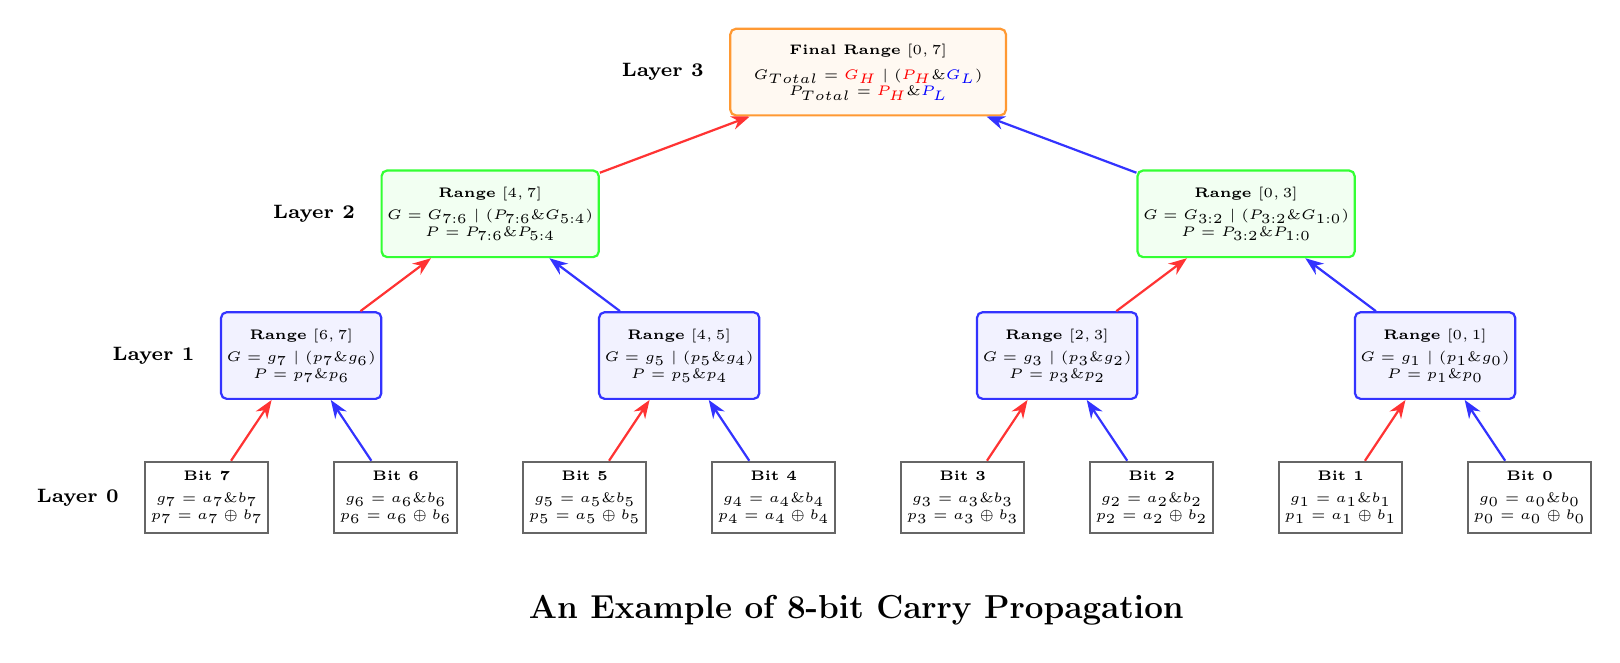
\begin{tikzpicture}[
    x=1.5cm, y=1.2cm, 
    node distance=1.5cm,
    leaf/.style={
        rectangle, 
        draw=black!60, 
        thick, 
        fill=white, 
        minimum width=1.35cm, 
        minimum height=0.9cm,
        font=\bfseries\tiny,  
        align=center,
        inner sep=2pt
    },
    mergebox/.style={
        rectangle, 
        draw=blue!80, 
        fill=blue!5, 
        thick, 
        rounded corners=2pt,
        minimum width=1.8cm, 
        minimum height=1.1cm,
        align=center,
        font=\tiny, 
        inner sep=2pt
    },
    arrow/.style={
        ->, 
        >=Stealth, 
        thick, 
        color=gray!70
    }
]

\foreach \i in {7,6,...,0} {
    \node[leaf] (b\i) at ({(7-\i)*1.6}, 0) {
        Bit \i\\[2pt]
        $g_{\i} = a_{\i} \& b_{\i}$\\
        $p_{\i} = a_{\i} \oplus b_{\i}$
    };
}
\node[left=0.2cm of b7, font=\bfseries\scriptsize, align=right] {Layer 0};

\foreach \i in {7,5,3,1} {
    \pgfmathparse{int(\i-1)}
    \let\j\pgfmathresult
    
    \node[mergebox] (L1_\i) at ($(b\i)!0.5!(b\j) + (0, 1.5)$) {
        \textbf{Range} $[\j, \i]$\\[2pt]
        $G = g_{\i} \mid (p_{\i} \& g_{\j})$\\
        $P = p_{\i} \& p_{\j}$
    };
    
    \draw[arrow, red!80] (b\i) -- (L1_\i);
    \draw[arrow, blue!80] (b\j) -- (L1_\i);
}
\node[left=0.2cm of L1_7, font=\bfseries\scriptsize, align=right] {Layer 1};

\node[mergebox, fill=green!5, draw=green!80] (L2_7) at ($(L1_7)!0.5!(L1_5) + (0, 1.5)$) {
    \textbf{Range} $[4, 7]$\\[2pt]
    $G = G_{7:6} \mid (P_{7:6} \& G_{5:4})$\\
    $P = P_{7:6} \& P_{5:4}$
};
\draw[arrow, red!80] (L1_7) -- (L2_7);
\draw[arrow, blue!80] (L1_5) -- (L2_7);

\node[mergebox, fill=green!5, draw=green!80] (L2_3) at ($(L1_3)!0.5!(L1_1) + (0, 1.5)$) {
    \textbf{Range} $[0, 3]$\\[2pt]
    $G = G_{3:2} \mid (P_{3:2} \& G_{1:0})$\\
    $P = P_{3:2} \& P_{1:0}$
};
\draw[arrow, red!80] (L1_3) -- (L2_3);
\draw[arrow, blue!80] (L1_1) -- (L2_3);

\node[left=0.2cm of L2_7, font=\bfseries\scriptsize, align=right] {Layer 2};

\node[mergebox, fill=orange!5, draw=orange!80, minimum width=3.5cm] (L3_7) at ($(L2_7)!0.5!(L2_3) + (0, 1.5)$) {
    \textbf{Final Range} $[0, 7]$\\[3pt]
    $G_{Total} = \textcolor{red}{G_{H}} \mid (\textcolor{red}{P_{H}} \& \textcolor{blue}{G_{L}})$\\
    $P_{Total} = \textcolor{red}{P_{H}} \& \textcolor{blue}{P_{L}}$
};
\draw[arrow, red!80] (L2_7) -- (L3_7);
\draw[arrow, blue!80] (L2_3) -- (L3_7);

\node[left=0.2cm of L3_7, font=\bfseries\scriptsize, align=right] {Layer 3};

\node[font=\bfseries\large, align=center] at (5.5, -1.2) {An Example of 8-bit Carry Propagation};

\end{tikzpicture}}
\vspace{10pt}\\
With \textbf{G} signifying local carry creation and \textbf{P} signifying carry transmission, the algorithm employs recursive doubling to merge carry information, achieving a time complexity of $O(\log W)$.
\vspace{3pt}
\begin{lstlisting}[language=C++]
int32_t add (int32_t a, int32_t b)
{
    int32_t p = a ^ b, g = a & b;
    g |= (p & (g << 1));p &= (p << 1);
    g |= (p & (g << 2));p &= (p << 2);
    g |= (p & (g << 4));p &= (p << 4);
    g |= (p & (g << 8));p &= (p << 8);
    g |= (p & (g << 16)); 
    return (a ^ b) ^ (g << 1);
}
\end{lstlisting}
\newpage
\subsection{Subtraction}
As established in the derivation of two's complement arithmetic in Section~1.2, the subtraction $a - b$ can be transformed into $a + (-b) = a + (\sim b + 1)$. 
\vspace{3pt}\\
By utilizing the already implemented \texttt{add} function, subtraction is therefore reduced to a constant number of bitwise operations, achieving $O(\log W)$ time complexity.
\vspace{3pt}
\begin{lstlisting}[language=C++]
int32_t subtract (int32_t a, int32_t b)
{
    return add (a, add (~b, 1));
}
\end{lstlisting}

\subsection{Multiplication}
The multiplication algorithm adapts traditional \textbf{column multiplication} to binary arithmetic. Analogous to shifting partial products in decimal, the binary multiplicand $a$ is left-shifted for each active bit in the multiplier $b$.
\vspace{3pt}\\
Let $b$ be represented in binary form as $b = \sum\limits_{i=0}^{W-1} b_i \cdot 2^i$, where $b_i \in \{0, 1\}$ is the $i$-th bit of $b$. Substituting this into the product $a \times b$ yields:
\[
a \times b = a \times \sum_{i=0}^{W - 1} (b_i \cdot 2^i) = \sum_{i=0}^{W - 1} b_i \cdot (a \cdot 2^i)
\]
\vspace{3pt}\\
Before computation, signed operands are converted to their absolute values. To prevent signed integer overflow (e.g., $\texttt{INT\_MIN}$), operands are cast to $\texttt{uint32\_t}$.
\vspace{3pt}\\
The algorithm achieves a time complexity of \textbf{$O(W \log W)$} (Both $\texttt{add ()}$ and $\texttt{subtract ()}$ have a time complexity of $O(\log W)$).
\vspace{8pt}
\begin{lstlisting}[language=C++]
int32_t multiply (int32_t a, int32_t b)
{
    int32_t sign = 0;
    uint32_t tmpa = static_cast <uint32_t> (a);
    uint32_t tmpb = static_cast <uint32_t> (b);
    uint32_t tmpres = 0;
    if (tmpa >> 31 & 1) 
    {
        tmpa = subtract (0, tmpa);
        sign ^= 1;
    }
    if (tmpb >> 31 & 1)
    {
        tmpb = subtract (0, tmpb);
        sign ^= 1;
    }
    while (tmpb)
    {
        if (tmpb & 1) tmpres = add (tmpres, tmpa);
        tmpa <<= 1;tmpb >>= 1;
    }
    int32_t res = static_cast <int32_t> (tmpres);
    if (sign) res = subtract (0, res);
    return res;
}
\end{lstlisting}
\newpage
\subsection{Division}
Similar to the multiplication algorithm, the sign bit is processed separately by converting both operands to absolute values (using $\texttt{uint32\_t}$ is necessary). 
\vspace{3pt}\\
According to \textbf{Euclidean Division Theorem}, the operation is expressed as $a = b \cdot q + r$, where $0 \le r < b$. Let quotient $q$ be represented in binary form as $q = \sum\limits_{i=0}^{W - 1} q_i \cdot 2^i$, where $q_i \in \{0, 1\}$ is the $i$-th bit of $q$. To determine the coefficients $q_i$, a \textbf{Greedy Strategy} is employed:
\begin{itemize}
  \item \textbf{case 1} $a < b \cdot 2^i$ \quad $b \cdot 2^i$ is too large to fit in the remainder, which implies $q_i = 0$.
  \item \textbf{case 2} $a \ge b \cdot 2^i$ \quad It implies $q_i = 1$. The $i$-th bit of the result is set, and the remainder is updated to $a \leftarrow a - b \cdot 2^i$.

  \textbf{Proof} 
  \vspace{3pt}\\
  Suppose that $q_i$ is set to 0 despite the condition $a \ge b \cdot 2^i$. 
  \vspace{3pt}\\
  The value of $r$ would satisfy the inequaity:
  \[r = a - \sum_{j=0}^{i-1} q_j \cdot b \cdot 2^j \ge a - b(2^i - 1)\]
  Substituting the condition $a \ge b \cdot 2^i$ into the inequality:
  \[r \ge b \cdot 2^i - b(2^i - 1) = b\]
  This leads to $r \ge b$, which contradicts the Euclidean division constraint $0 \le r < b$.
\end{itemize}
The comparison outlined in Section~1.3 should be utilized to avoid invalid behaviors. And the algorithm achieves a time complexity of \textbf{$O(W \log W)$}.
\vspace{8pt}
\begin{lstlisting}[language=C++]
int32_t divide (int32_t a, int32_t b)
{
    int32_t sign = 0;
    uint32_t tmpa = static_cast <uint32_t> (a);
    uint32_t tmpb = static_cast <uint32_t> (b);
    uint32_t tmpres = 0;
    if (tmpa >> 31 & 1) 
    {
        tmpa = subtract (0, tmpa);
        sign ^= 1;
    }
    if (tmpb >> 31 & 1)
    {
        tmpb = subtract (0, tmpb);
        sign ^= 1;
    }
    for (int i = 31;~i;--i)
    {
        int32_t diff = subtract (tmpa >> i, tmpb);
        if (!(diff >> 31 & 1))
        {
            tmpres |= (1 << i);
            tmpa = subtract (tmpa, tmpb << i);
        }
    }
    int32_t res = static_cast <int32_t> (tmpres);
    if (sign) res = subtract (0, res);
    return res;
}
\end{lstlisting}
\newpage
\subsection{Modulo}
In mathematical number theory, the modulo operation is defined as $a \bmod b = a - b \cdot \lfloor \frac{a}{b} \rfloor$. But in C++, the modulo operation follows the \textbf{truncate toward zero} rule.
\vspace{3pt}
Note that the $\texttt{divide (a,b)}$ is also implemented to align with this C++ standard (truncate toward zero rule), the Euclidean relation $a = qb + r$ can be reversed to derive the correct modulus $r = a - qb$.
\vspace{3pt}
The time complexity of this algorithm is \textbf{$O(W \log W)$}.
\vspace{8pt}
\begin{lstlisting}[language=C++]
int32_t modulo (int32_t a, int32_t b)
{
    int32_t q = divide (a, b);
    int32_t mx = multiply (b, q);
    return subtract (a, mx);
}
\end{lstlisting}
\section{Unit Test}

Following initial verification, serveral test cases were rigorously enhanced with LLM (prompts in Appendix) to focus on three critical dimensions:

\subsection{Boundary Value Analysis}
\begin{itemize}
    \item \textbf{Extremes}: Operations involving \texttt{INT\_MAX} and \texttt{INT\_MIN}.
    \item \textbf{Zero Handling}: Rigorous testing of $0$ as both an operand and a result 
    \end{itemize}

\subsection{Randomized Mixed-Sign Testing}
\begin{itemize}
    \item \textbf{Full-Range Inputs}: Random integers selected from the entire \texttt{int32\_t} range.
    \item \textbf{Mixed Signs}: Combinations of positive and negative to ensure correctness.
\end{itemize}

\subsection{Truncation and Sign Consistency}
The tests rigorously verify the sign correctness for all four permutations of input signs: $a \bmod b$, $a \bmod (-b)$, $(-a) \bmod b$ and $(-a) \bmod (-b)$.

\subsection{Flow Test}
A dedicated suite of flow tests was designed to verify the implementation's behavior under overflow and underflow conditions.
\newpage
\section{Appendix}
It is hereby declared that Generative AI tools were utilized in this project to assist with code optimization, report polishing, and test case generation. The core logic and implementation were verified by the author. $\textbf{Representative excerpts}$ of the interaction are provided below:
\begin{description}
    \item[Report Translation and Polishing] \hfill \\
    \begin{figure}[htbp]
    \center
    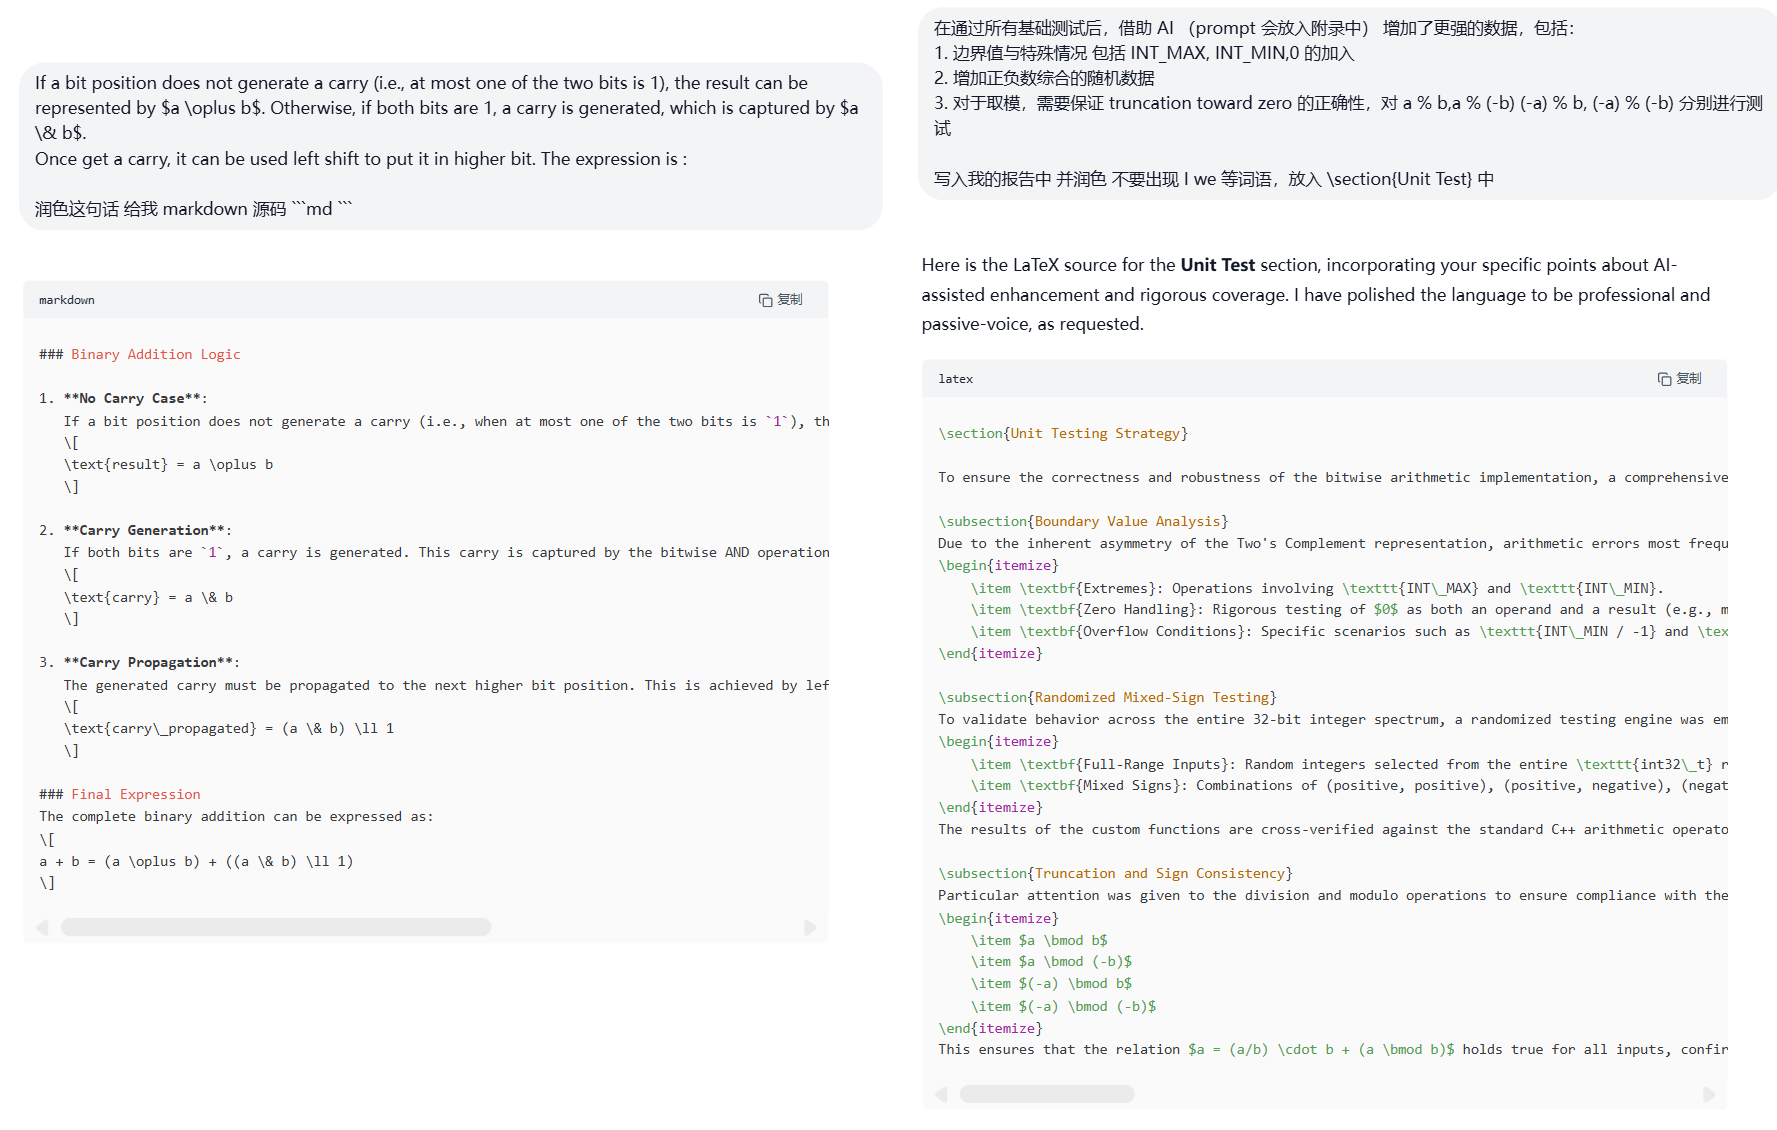
\includegraphics[width=0.9\textwidth]{pic/1.png}
    \end{figure}
    \item[Add Content] \hfill \\
    \begin{figure}[htbp]
    \center
    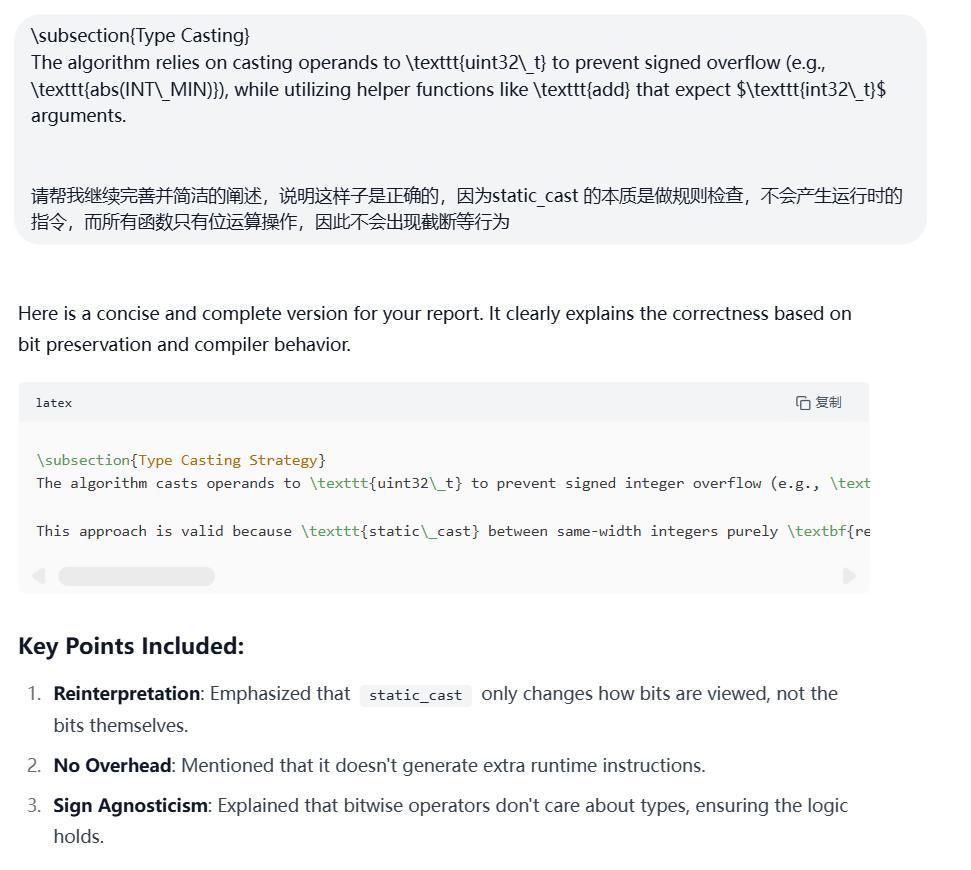
\includegraphics[width=0.6\textwidth]{pic/2.png}
    \end{figure}
    \newpage
    \item[Test Case Enhancement] \hfill \\
    \begin{figure}[htbp]
    \center
    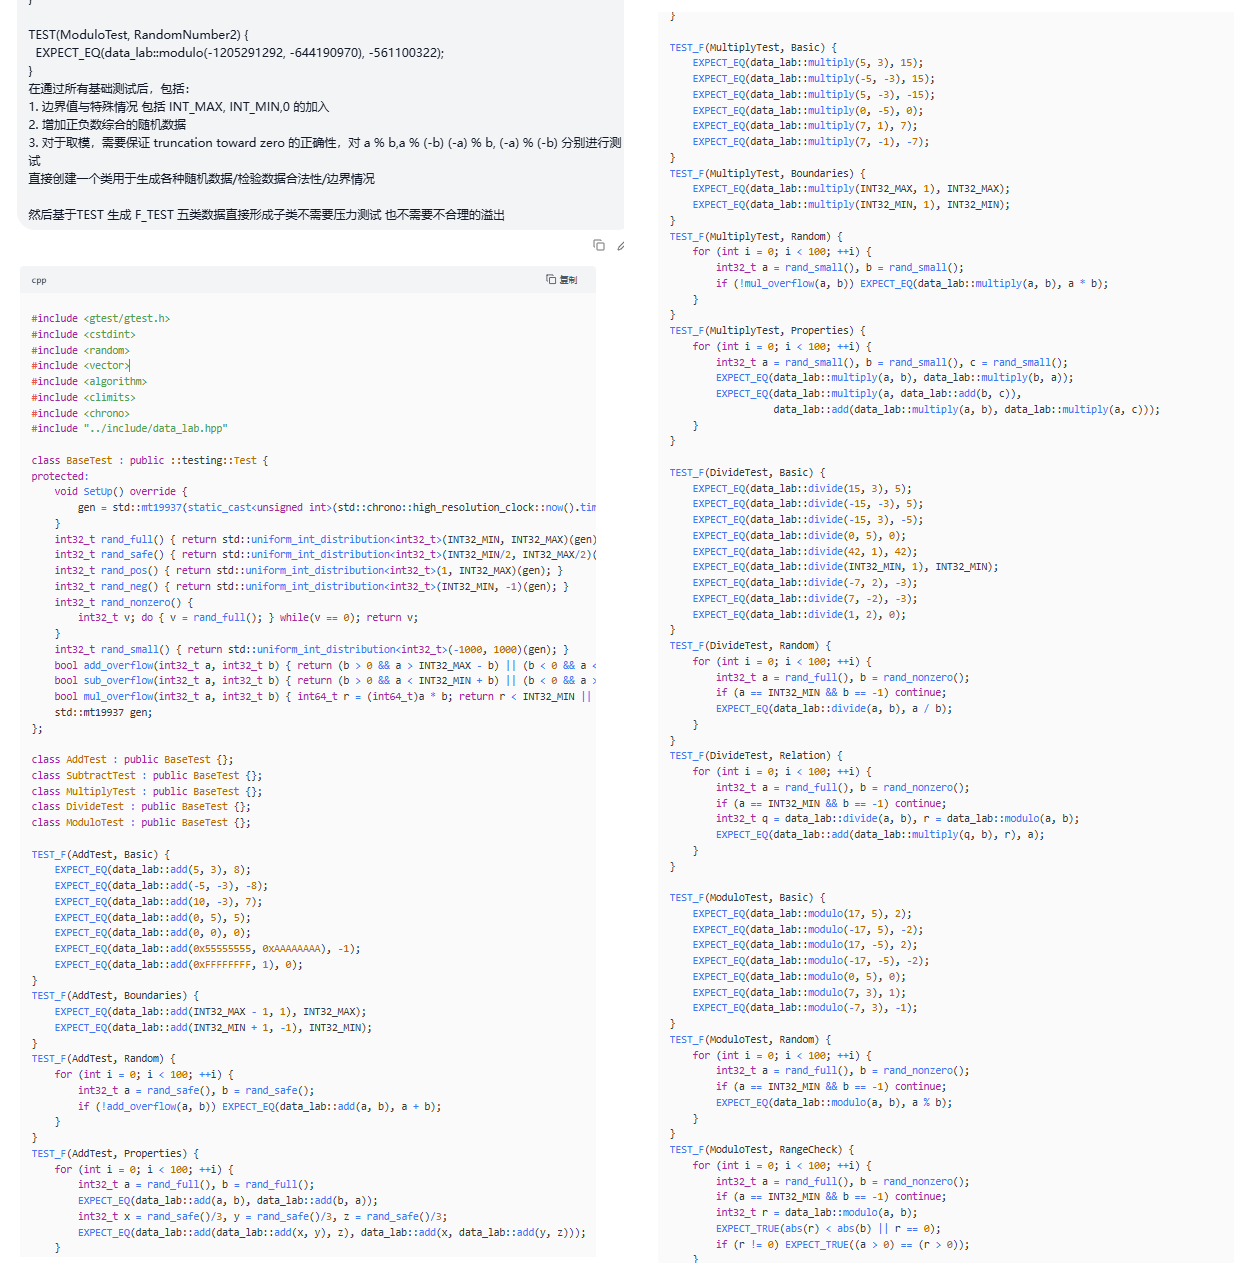
\includegraphics[width=0.9\textwidth]{pic/3.png}
    \end{figure}
    \newpage
    \item[Auxiliary Image Generation] \hfill \\
    This diagram is the final result of implementing the illustration in Section ~2.1, synthesized after multiple rounds of prompt refinement.
    \begin{figure}[htbp]
    \center
    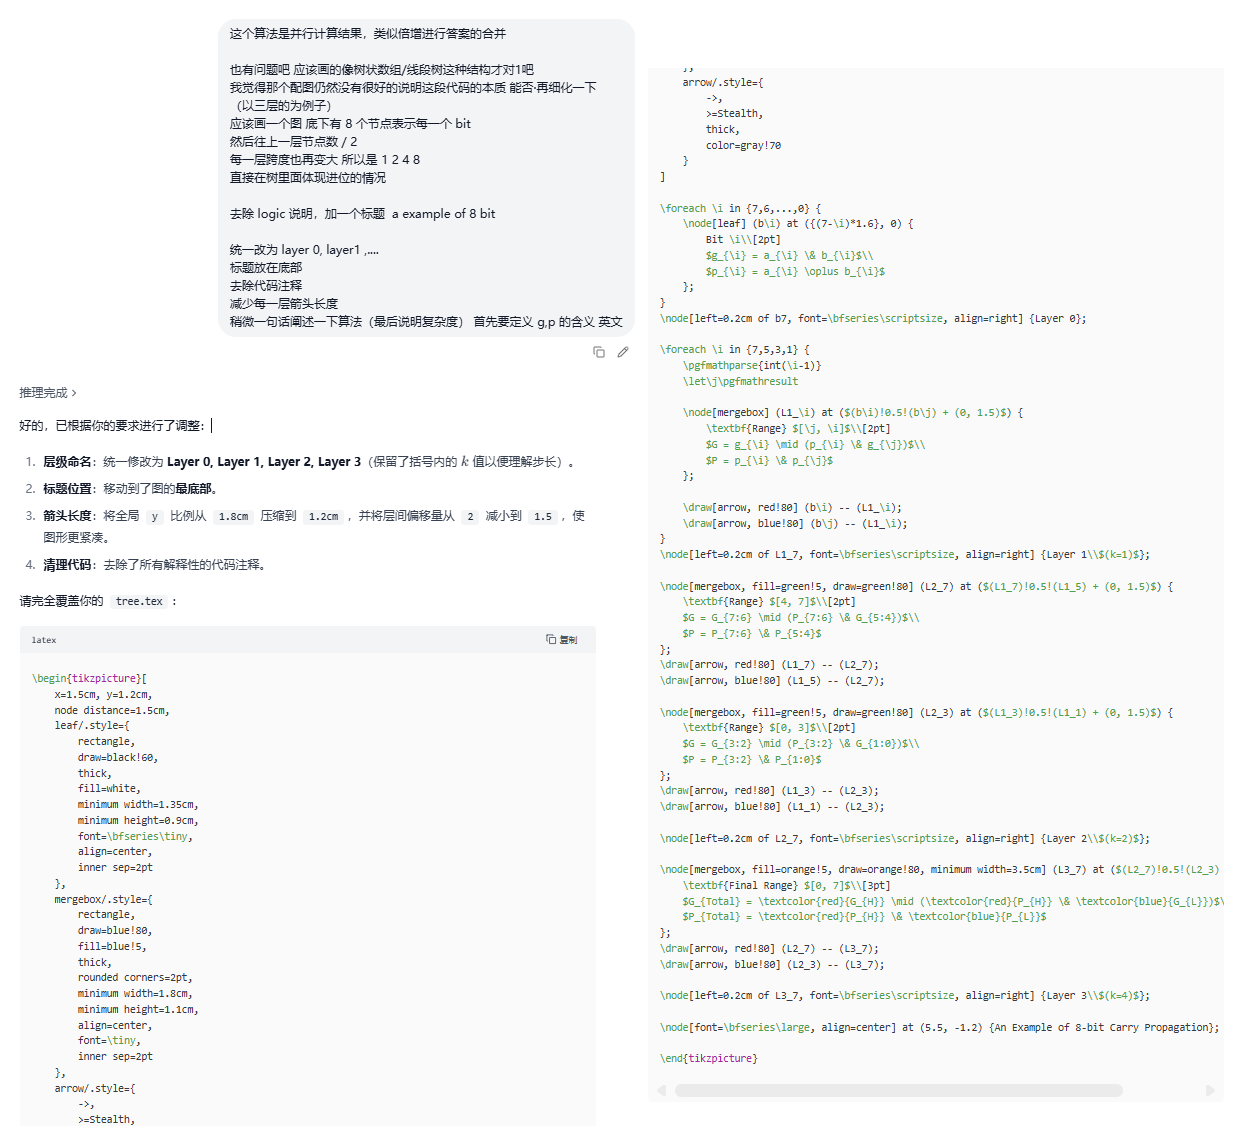
\includegraphics[width=0.9\textwidth]{pic/4.png}
    \end{figure}
    \item[Problem Assistance] \hfill \\
    \item[] \begin{figure}[htbp]
    \center
    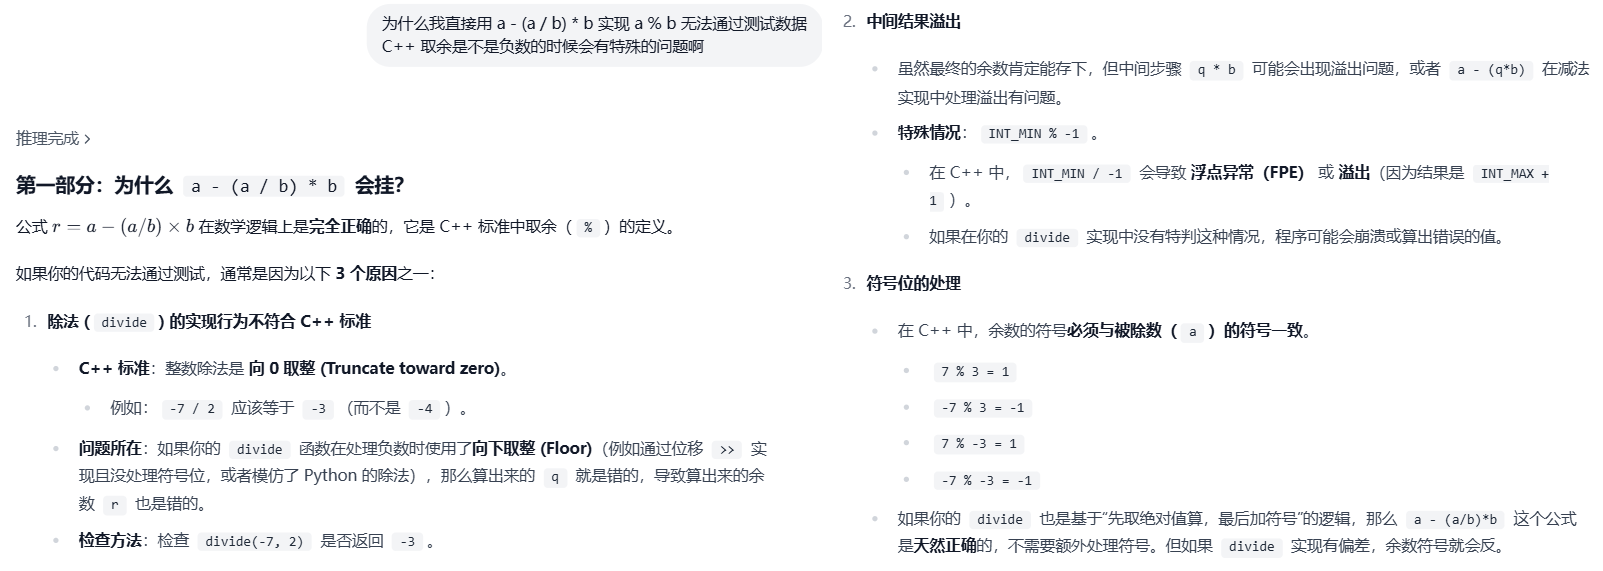
\includegraphics[width=0.9\textwidth]{pic/5.png}
    \end{figure}
    \item[\textbf{Other Links}] \hfill\\
    \href{https://chat.deepseek.com/share/51tjehjaw7r9yq9fy3}{Link1}
    \href{https://chat.deepseek.com/share/vqq765x7efbo1ibs98}{Link2}
    \href{https://chat.deepseek.com/share/uhx21hfsh5u19q99j8}{link3}

\end{description}
\end{document}